                                                                               \documentclass[tikz]{standalone}
\usepackage{lmodern}
\usepackage[algoruled,vlined,linesnumbered,titlenotnumbered,noend]{algorithm2e}
\usepackage{color,amsmath,bm,bbm,stmaryrd,amssymb,pifont,bbding}
\usetikzlibrary{backgrounds}
\usetikzlibrary{calc} 

\usetikzlibrary{shapes}
\usetikzlibrary{shadows}
\usetikzlibrary{decorations.pathmorphing}
\usetikzlibrary{decorations.text}
\usetikzlibrary{decorations}
\usetikzlibrary{arrows,bending}
\usetikzlibrary{shapes.arrows}
\tikzset{nobg/.style={show background rectangle,background rectangle/.style={opacity=0}}}


\input ../../styles
\input ../../globalcomm
\usetikzlibrary{arrows, shapes.gates.logic.US, calc}

\begin{document}


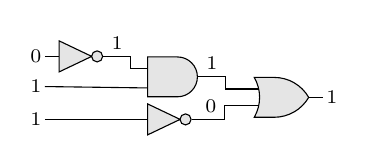
\begin{tikzpicture}

\node[and gate US, draw,name=and,anchor=north west,logic gate inputs=nn,fill=gray!20] 
at (0,0){};
\node[not gate US, draw,name=not1,anchor=east,fill=gray!20] at
($(and.north west)+(-20pt,0pt)$) {};
\node[or gate US, draw,name=or,anchor=north west,logic gate inputs=nn,fill=gray!20] at ($(and.east) + (20pt,0pt)$) {};


\node[name=i1,anchor=east,inner sep=1pt,font=\scriptsize] at ($(not1.west)+(-5pt,0pt)$) {$0$};
\node[name=i2,anchor=north,inner sep=1pt,font=\scriptsize] at (i1.south|-and.west) {$1$};
\node[name=i3,anchor=north,inner sep=1pt,font=\scriptsize] at ($(i2.south)+(0pt,-5pt)$) {$1$};
\node[name=out,anchor=west,inner sep=1pt,font=\scriptsize] at ($(or.east)+(5pt,0pt)$) {$1$};

\node[not gate US, draw,name=not2,anchor=west,fill=gray!20] at
(and.west |- i3.west) {};


\draw (not1.output) -- node[above=-1pt,font=\scriptsize]{$1$}($(not1.output)+(10pt,0pt)$) |- ($(and.west)+(0pt,3pt)$);
\draw (and.output) -- node[above=-1pt,font=\scriptsize]{$1$}($(and.output)+(10pt,0pt)$) |- ($(or.west)+(0pt,3pt)$);
\draw (not2.output) -- node[xshift=1pt,above=-1pt,font=\scriptsize]{$0$}($(not2.output)+(12pt,0pt)$) |- ($(or.west)+(0pt,-3pt)$);
\draw (i1) -- (not1);
\draw (i2) -- ($(and.west)+(0pt,-4pt)$);
\draw (i3) -- (not2);
\draw (or.output) -- (out);
    
\end{tikzpicture}


\end{document}

